\documentclass[border=3pt]{standalone}
\usepackage[T1]{fontenc}
\usepackage[utf8]{inputenc}
\usepackage{lmodern}
\usepackage{amsmath,amssymb}
\usepackage{xcolor}
\usepackage{tikz}
\usepackage{fontawesome5}
\usepackage{ragged2e}
\usetikzlibrary{shapes,shapes.geometric,shapes.misc,arrows.meta,positioning,
                calc,fit,backgrounds,decorations.pathreplacing,
                decorations.markings,patterns,chains}
\usetikzlibrary{decorations.pathreplacing,decorations.markings}
\definecolor{primary}{HTML}{1A5276}
\definecolor{secondary}{HTML}{2E86C1}
\definecolor{accent}{HTML}{E74C3C}
\definecolor{lightbg}{HTML}{EBF5FB}
\definecolor{defbg}{HTML}{FDF2E9}
\definecolor{greenhl}{HTML}{27AE60}
\definecolor{purplehl}{HTML}{8E44AD}
\definecolor{goldhl}{HTML}{B7950B}
\definecolor{tealhl}{HTML}{117A65}
\definecolor{codebg}{HTML}{F4F6F7}
\definecolor{neutral}{HTML}{707B7C}
\definecolor{dom1}{HTML}{1F618D}
\definecolor{dom2}{HTML}{117864}
\definecolor{dom3}{HTML}{6C3483}
\definecolor{dom4}{HTML}{922B21}
\definecolor{dom5}{HTML}{B7950B}
% --- carried over from ccna.sty so figures match the book exactly
\tikzset{
  dev/.style={rounded corners=3pt, draw=#1, fill=#1!8, text=#1!45!black,
              line width=0.9pt, minimum width=1.45cm, minimum height=1.05cm,
              align=center, font=\scriptsize\bfseries, inner sep=2pt},
  wirestyle/.style={line width=0.9pt, neutral!75},
  xconn/.style={line width=0.9pt, neutral!75, dash pattern=on 2.5pt off 2pt},
}

\newcommand{\Rtr}[3]{\node[dev=dom3] (#1) at #2 {\faIcon{route}\\#3};}
\newcommand{\Sw}[3]{\node[dev=dom2] (#1) at #2 {\faIcon{sitemap}\\#3};}
\newcommand{\Msw}[3]{\node[dev=dom3] (#1) at #2 {\faIcon{layer-group}\\#3};}
\newcommand{\Host}[3]{\node[dev=neutral] (#1) at #2 {\faIcon{desktop}\\#3};}
\newcommand{\Lap}[3]{\node[dev=neutral] (#1) at #2 {\faIcon{laptop}\\#3};}
\newcommand{\Srv}[3]{\node[dev=dom1] (#1) at #2 {\faIcon{server}\\#3};}
\newcommand{\Ap}[3]{\node[dev=dom5] (#1) at #2 {\faIcon{wifi}\\#3};}
\newcommand{\Wlc}[3]{\node[dev=dom5] (#1) at #2 {\faIcon{broadcast-tower}\\#3};}
\newcommand{\Fw}[3]{\node[dev=dom4] (#1) at #2 {\faIcon{shield-alt}\\#3};}
\newcommand{\Cld}[3]{\node[dev=neutral] (#1) at #2 {\faIcon{cloud}\\#3};}
\newcommand{\Phone}[3]{\node[dev=dom5] (#1) at #2 {\faIcon{phone-alt}\\#3};}
\newcommand{\Prn}[3]{\node[dev=neutral] (#1) at #2 {\faIcon{print}\\#3};}

% A link. The optional argument takes tikz options (e.g. xconn for a
% trunk drawn dashed); the fourth argument labels the link.
\newcommand{\wire}[4][wirestyle]{%
  \draw[#1] (#2) -- node[font=\tiny, text=neutral!85!black, fill=white,
                          inner sep=1.2pt, midway] {#4} (#3);}
\newcommand{\plainwire}[3][wirestyle]{\draw[#1] (#2) -- (#3);}


\newenvironment{topology}[1][]
  {\begin{center}\begin{tikzpicture}[font=\scriptsize,#1]}
  {\end{tikzpicture}\end{center}}


\newcommand{\cmd}[1]{\texttt{\small #1}}
\newcommand{\term}[1]{\textbf{\textcolor{primary}{#1}}}
\newcommand{\chref}[1]{Chapter~\ref{ch:#1}}
\newcommand{\ccnafitw}[1]{#1}
\providecommand{\thefigure}{}
% --- progressive builds
\newcount\buildlevel \buildlevel=99
% \stepvis{n}{..} appears from level n onward; \steponly{n}{..} at
% level n alone, which is how a caption is swapped rather than
% accumulated as the build advances. \stepdim{n}{..} is the
% complement of \stepvis: it shows only BEFORE level n, so a
% pair of them draws an element faint and then solid. That keeps
% the canvas full from step 1, which matters for a figure whose
% shape is itself the lesson -- a five-rung ladder revealed one
% rung at a time leaves a void where the method should be.
\newcommand{\stepvis}[2]{\ifnum#1>\buildlevel\relax\else#2\fi}
\newcommand{\steponly}[2]{\ifnum#1=\buildlevel #2\fi}
\newcommand{\stepdim}[2]{\ifnum#1>\buildlevel #2\fi}
% Slide text does not hyphenate. A projected caption broken as
% ``uni-cast'' costs the reader a beat that print can afford and a
% lecture cannot, and the ragged edge it avoids is invisible at
% four metres anyway.
\hyphenpenalty=10000 \exhyphenpenalty=10000
\begin{document}
\buildlevel=1
% Slide build of Figure 12.1 -- one triangle that evolves, not two side by side.
%
%   1  three switches, three cables: physically redundant, and fine
%   2  one broadcast starts going round, and nothing stops it
%   3  spanning tree blocks one port -- the cable is still there
%
% The cable that gets blocked stays drawn at every level, so Morph recolours
% it rather than removing and re-adding it. That is the point the caption
% makes: spanning tree does not remove redundancy, it holds it in reserve.
\begin{tikzpicture}[font=\scriptsize]
  \tikzset{
    dv/.style={rounded corners=3pt, draw=#1, fill=#1!8, text=#1!45!black,
               line width=1.1pt, minimum width=1.8cm, minimum height=1.2cm,
               align=center, font=\small\bfseries},
    w/.style={line width=1.4pt, neutral!70},
    % text width is not optional: without it the caption is one long line
    % that runs past the pinned bounding box and is cropped.
    capt/.style={font=\bfseries, anchor=north west, text width=9.4cm,
                 align=left}}

  \useasboundingbox (-1.0,-2.6) rectangle (9.6,3.0);

  \node[dv=dom2] (a) at (4.0,2.0) {\faIcon{sitemap}\\SW1};
  \node[dv=dom2] (b) at (1.9,-0.1) {\faIcon{sitemap}\\SW2};
  \node[dv=dom2] (c) at (6.1,-0.1) {\faIcon{sitemap}\\SW3};

  \draw[w] (a) -- (b);
  \draw[w] (a) -- (c);
  % the third cable: drawn at every level, recoloured at level 3 so Morph
  % changes its colour rather than removing and re-adding the shape
  \ifnum\buildlevel<3
    \draw[w] (b) -- (c);
  \else
    \draw[w, accent!70, dash pattern=on 4pt off 3pt] (b) -- (c);
  \fi

  \steponly{1}{\node[capt, text=neutral!45!black] at (-0.6,-1.5)
      {Three switches, three cables. The redundancy is deliberate.};}

  \steponly{2}{%
    % An arc, not a circle: TikZ draws no arrowhead on a closed path, so a
    % \draw[->] ... circle renders a plain ring with no sense of direction.
    \draw[-{Stealth[length=3.2mm]}, accent!85, line width=2.2pt]
        (4.72,0.62) arc (0:308:0.72);
    \node[capt, text=accent!75!black] at (-0.6,-1.5)
        {One broadcast, and an Ethernet frame has no TTL --- it circulates
         for ever.};}

  \steponly{3}{%
    \node[circle, draw=accent!85, fill=white, line width=1.4pt,
          inner sep=2pt, font=\tiny\bfseries, text=accent!75!black]
        at (4.0,-0.1) {BLK};
    \node[font=\small\bfseries, text=dom2!45!black, anchor=west]
        at (5.05,2.0) {ROOT};
    \node[capt, text=dom2!50!black] at (-0.6,-1.5)
        {One port blocks. The cable is still there, ready if another
         link fails.};}
\end{tikzpicture}

\end{document}
